\documentclass[rnd]{mas_proposal}
% \documentclass[thesis]{mas_proposal}

\usepackage[utf8]{inputenc}
\usepackage{amsmath}
\usepackage{amsfonts}
\usepackage{amssymb}
\usepackage{graphicx}
\usepackage{pgfgantt}
\title{Interactive Reinforcement Learning with Human Feedback Collected through VR Headsets}
\author{Behrouz Ghamkhar}
\supervisors{Prof. Dr. Teena Chakkalayil Hassan\\Mr. Michal Stolarz}
\date{September 2025}

% \thirdpartylogo{path/to/your/image}

\begin{document}

\maketitle

\pagestyle{plain}

\section{Introduction}

\subsection{Topic of This R\&D Project}
Robots have the potential to become important partners in human environments, helping with tasks at home or in complex collaborative work \citep{Chetouani2021, Akalin2021}. However, it is still very difficult for robots to work well in open-world environments. These environments have unknown tasks, new objects, and dynamic human interactions. This gap highlights an important shortcoming: robots often lack the common sense and contextual understanding that humans use effortlessly to generalize their skills and interpret underspecified instructions.

A promising way to address this problem is Interactive Reinforcement Learning (IRL), which includes human feedback directly into the robot's learning loop. \citep{Lin2020, BradleyKnox2008}. This approach aims to improve sample efficiency, accelerate policy acquisition, and align the robot's behavior with human preferences and intentions \citep{Lin2020}. By learning from evaluative feedback, demonstrations, or advice, IRL agents can adapt to complex, real-world constraints more effectively than autonomous reinforcement learning agents relying only on engineered reward functions.

Despite its potential, a significant bottleneck in traditional IRL is the interface for human feedback. Most systems rely on low-bandwidth, explicit channels such as keyboard presses, button clicks, or simple GUI interactions \citep{Faulkner2020, Loftin2014}. These methods are unnatural and awkward for the human teacher. They also cannot capture the rich details of human communication, like gestures, gaze, and tone of voice \citep{9794595, Lin2020a}. This creates an expressiveness gap, limiting the quality and type of information that can be transferred from human to robot.

At the same time, advances in consumer-grade Virtual Reality (VR) technology have created new opportunities for human-computer interaction. Modern VR headsets have many sensors that can track head pose, hand gestures, eye gaze, and voice input, offering an immersive and intuitive interface for human communication. These sensors can capture detailed human feedback in a natural way \citep{Winkler2022,Luo2024}. Even with this potential, VR and IRL have mostly developed separately. VR is often used to collect demonstration data (e.g., \citep{10904309, Mosbach2022}) and a recent study used it for preference-based learning \citep{Heuvel2025}. However, using VR to collect real-time scalar feedback as part of an IRL system is still unexplored.

This project aims to close this gap by developing a novel IRL system that uses VR as an interface for human feedback. The core idea is to allow users to interact with a virtual agent using gestures, gaze, voice, or controller inputs to deliver reinforcement signals in real time. However, a key challenge is scalability: a human cannot be expected to wear a VR headset for the millions of iterations a typical RL agent needs to learn. To solve this, we propose a two-stage approach: first, we collect a high-quality dataset of human feedback within targeted VR scenarios; second, we use this dataset to train a predictive feedback model that learns to imitate the human's feedback patterns based on the agent’s behavior. This model will then be integrated into the RL loop to provide scalable and consistent feedback. In this way, the IRL process can be supported and scaled.

The main goal and contribution of this research is to build a new way of human-in-the-loop RL by using immersive technologies. This should make AI training more efficient, natural, and human-centered.


\subsection{Relevance of This R\&D Project}
This project is important for several reasons:

\textbf{Scientific Value:} This work is among the first to integrate rich, multi-modal feedback from VR headsets—such as pose, gaze direction, and hand gestures—into the IRL feedback loop. It goes further than simple binary or scaler inputs \citep{Faulkner2020, Loftin2014} and makes it possible to give continuous and context-aware feedback, opening new research directions at the intersection of immersive interfaces and machine learning.

\textbf{Practical Impact:} The outcomes of this project will directly benefit applications that require efficient and intuitive human-in-the-loop training. In robotics, for example, it can reduce the number of required demonstrations by an estimated 30–50\% by supplementing them with rich feedback, accelerating policy learning for tasks such as dexterous manipulation \citep{Christen2019}. In the simulation and digital twin industry, animators and designers could use this system to create more realistic and responsive virtual characters \citep{Winkler2022, Luo2024} with less manual effort. Domain experts—such as rehabilitation therapists or simulation designers—will be able to train agents more naturally and effectively, without requiring programming expertise.

\textbf{Technological Advancement:} The project will deliver a framework that connects popular VR development platforms (e.g., Unity engine) with standard RL libraries (e.g., PyTorch, RLlib). It will also provide useful infrastructure  that allows other researchers to build upon our work and encourage collaboration in the community. By providing both a practical toolkit and a dataset of VR-human feedback, we aim to lower the barrier to entry for future studies in immersive human–agent interaction.

\section{Related Work}

\subsection{Reinforcement Learning}
Reinforcement Learning (RL) is a machine learning paradigm where an autonomous agent learns to make sequential decisions by interacting with an environment. The core objective is to learn a policy—a mapping from states of the environment to actions—that maximizes a numerical reward signal over time \citep{Lin2020}. This interaction is formally modeled as a Markov Decision Process (MDP), defined by the tuple $(S, A, P, R, \gamma)$, where:

\begin{itemize}
    \item $S$ is a set of states,
    \item $A$ is a set of actions,
    \item $P(s_{t+1} | s_t, a_t)$ is the state transition probability,
    \item $R(s_t, a_t, s_{t+1})$ is the reward function, and
    \item $\gamma \in [0, 1]$ is a discount factor that weights the importance of immediate versus future rewards.
\end{itemize}

The agent's goal is to learn an optimal policy $\pi^*(a|s)$ that maximizes the expected cumulative discounted reward, or return. A fundamental concept is the value function $V^{\pi}(s)$, which estimates the expected return from state $s$ when following policy $\pi$, and the action-value function $Q^{\pi}(s, a)$, which estimates the expected return after taking action $a$ in state $s$ and thereafter following policy $\pi$.

A review of current research shows that IRL uses many different algorithms. Researchers choose these methods strategically based on the task and the type of human feedback available.

The algorithms used in human-robot interaction (HRI) can be divided into three main groups, each with different strengths:

\subsubsection {Value-Based Methods: Stability and Integration}
Value-based methods, especially Q-learning and its variants, are the most common type. They are popular because they are well-understood, stable in discrete action spaces, and it is straightforward to add human feedback to them.
\begin{itemize}
    \item Standard \& Contextual Q-Learning: The foundational tabular Q-learning algorithm is effectively employed in simpler, discrete state-action tasks, such as the sequential object selection task in \citet{9794595} and the grid-world navigation and trust optimization in \citet{Alzahrani2025}. Its simplicity makes the impact of human advice or reward shaping directly observable. \citet{MunguiaGaleano2023} uses a Contextual Q-learning (CQL) approach to leverage affordances, demonstrating how classic value-based methods can be extended for more complex, context-aware HRI.
    \item Deep Q-Networks (DQN): For higher-dimensional state spaces (e.g., pixel inputs in simulated environments), Deep Q-Networks are the natural evolution. \citet{Moreira2020} uses a DQN with a CNN for an object-sorting task, while \citet{Xu2021} develops a more advanced Bayesian Deep Q-Network (BDQN) to robustly integrate the uncertainty inherent in EEG-based implicit feedback. This shows a trend where value-based methods are scaled using deep learning while maintaining their core principle of learning an action-value function.
\end{itemize}


\subsubsection{Policy Search and Policy Gradient Methods: Direct Optimization}
Policy Search methods directly optimize the policy parameters. This approach is often chosen for continuous control tasks common in robotics, like manipulation and locomotion.
\begin{itemize}
    \item Policy Learning by Weighting Exploration with Returns (PoWER): This algorithm is a key part of policy search in robotics. \citet{8624972} uses PoWER in a latent space to learn a ball-throwing skill, demonstrating how policy search can be effectively guided by discrete human ratings instead of engineered rewards.
    \item Policy Gradient and Cross-Entropy Method: These are foundational policy optimization techniques. \citet{6147010} uses Policy Gradient and Cross-Entropy methods in their "Augmented RL" framework, showcasing their utility for online weight adaptation between human and environmental rewards. This highlights a key strength: the direct coupling between human feedback (which often critiques the policy) and the policy update rule.
\end{itemize}

\subsubsection{Actor-Critic and Advanced Methods} Complexity and Continuous Control
Actor-Critic methods, which combine value function and policy learning address complex, continuous control problems. Their ability to handle high-dimensional action spaces makes them suitable for modern robotic simulation.
\begin{itemize}
    \item Proximal Policy Optimization (PPO): A modern actor-critic algorithm known for its stability, PPO is used in several advanced physics-based simulation studies. It is used for human motion tracking and avatar control in \citet{Winkler2022}, \citet{Ye2022}, and \citet{Luo2024}. In these works, PPO is not typically interactive with a human during training but is used in an imitation learning setting, often trained on motion capture (MoCap) data, which can be seen as a form of offline human demonstration.
    \item Soft Actor-Critic (SAC): An algorithm that maximizes both expected return and entropy (promoting exploration), SAC is used by \citet{GonzalezSantocildes2024} for its sample efficiency and robustness in learning comfort-aware robot behaviors. Its off-policy nature makes it well-suited for learning from the potentially expensive data gathered in HRI experiments.
\end{itemize}


\subsubsection{Human-Feedback-Specific Frameworks}
A large part of the literature does not use a standard RL algorithm as its core. Instead, it builds a dedicated framework around human input.

\begin{itemize}
    \item TAMER (Training an Agent Manually via Evaluative Reinforcement): Introduced by \citet{BradleyKnox2008}, TAMER is a key framework that uses supervised learning to model a human's reward function from scalar feedback. It is not RL in the traditional sense but is a cornerstone of IRL. Its influence is clear in studies like \citet{Lin2020a}, which adapts its principles to interpret social feedback, and \citet{Faulkner2020}, which combines it with RL.
    \item Policy Shaping \& Algorithm-Agnostic Frameworks: Several studies, such as \citet{Faulkner2020} and \citet{KesslerFaulkner2021}, propose meta-frameworks like REPaIR and AMPS. These are designed to filter or interpret human feedback and can be layered on top of various underlying RL algorithms (often Q-learning or policy gradients), making them flexible tools for handling imperfect teachers.
\end{itemize}

A primary challenge in RL is the sample inefficiency in learning from sparse environmental rewards, which often requires millions of interactions for an agent to master complex tasks. This project addresses this issue by integrating human feedback to accelerate and guide the learning process, moving beyond traditional RL frameworks that rely only on manually designed reward functions.

\subsection{Survey of Related Work}
Our work sits at the intersection of IRL, HRI, and VR interfaces. We review key contributions across these domains.

\subsubsection{Interactive Reinforcement Learning (IRL)}
The foundation of this review is based on important papers that shaped the IRL field. Key work by \citet{BradleyKnox2008} introduced TAMER, showing that human evaluative feedback could train agents much faster than autonomous RL. This was extended into social domains by \citet{Lin2020a} and \citet{Lin2020} who provide a comprehensive review of IRL from human social feedback, distinguishing between evaluative feedback (e.g., rewards or punishments that signal approval or disapproval) and instructive feedback (e.g., advice, corrections, or demonstrations that guide the learner toward desired behaviors). 

A number of IRL frameworks have been proposed to integrate human feedback in different ways. The TAMER framework models human feedback as a reward signal that the agent learns to predict and use for policy improvement. This enables the agent to quickly adapt its behavior without relying on pre-defined environmental rewards \citet{BradleyKnox2008}.
COACH, in contrast, uses human feedback directly to calculate the policy gradient in an actor-critic algorithm. This allows for more flexible guidance, particularly in continuous action spaces, and supports real-time corrective feedback during learning \citep{Lin2020}.

Early work by \citet{6147010} explored augmented reinforcement learning for interaction with non-experts. A significant challenge in IRL is the quality of human input; \citet{Loftin2014} investigated using implicit human feedback strategies, while \citet{Faulkner2020} and \citet{KesslerFaulkner2021} developed specific algorithms for learning from inaccurate or imperfect teachers. The field has explored various feedback modalities, including haptics \citep{10490256} and even bio-signals, such as the use of EEG-based implicit human feedback to accelerate learning \citep{Xu2021}.

\subsubsection{VR for Data Collection and Demonstration}
The use of VR as a powerful tool for collecting human data for robot learning is well-established. A primary application has been in Learning from Demonstration (LfD) and robot programming, where methods range from multi-resolution corrective demonstration \citep{6225294} and learning responsive behavior by imitation \citep{6696819} to Bayesian fusion of multimodal advice \citep{9794595}. \citet{Christen2019} used motion capture data from human-human interactions to guide the reward function for training dexterous HRI policies. \citet{Mosbach2022} used GPU-based simulation and high-quality demonstrations, often collected in VR, to accelerate manipulation learning. More recently, \citet{10904309} developed RAMPA, a system using Augmented Reality for machine programming by demonstration, highlighting the trend towards immersive technologies for intuitive teaching. This approach is also used in neurorehabilitation, as shown by \citet{8009418}, who developed a learning-based agent for home therapy using EMG and avatar-based feedback.

\subsubsection{VR for Preference and Feedback}
While VR for demonstration is mature, its use for providing evaluative feedback is an emerging area. The most directly related work is by \citet{Heuvel2025}, who investigated the impact of VR and 2D interfaces on human feedback in \textit{preference-based} robot learning. Their work focuses on comparing interfaces for offline, comparative feedback. Our project aims to extend this line of inquiry into the domain of real-time, in-the-loop \textit{scalar} feedback, which is a distinct and unexplored challenge.

\subsubsection{Avatar and Motion Control in VR}
A critical technical challenge is interpreting the sparse sensor data from a VR headset into a meaningful representation of human state. This is an area of intense research in computer vision and graphics. Recent breakthroughs have employed Reinforcement Learning to create physically plausible avatars. \citet{Winkler2022} presented QuestSim, an RL framework that takes sparse signals from an HMD and two controllers to simulate full-body motion. This work was advanced by \citet{Luo2024}, who developed a method for a real-time simulated avatar from head-mounted sensors, a technology crucial for providing the context-aware feedback our system intends to use. Further foundational work includes that of \citet{Ye2022} on generating physically realistic full-body motion for VR users.

\subsubsection{Other Relevant Works}
Other relevant works include the integration of feedback in latent space for skill learning \citep{8624972}, the use of fairness-sensitive policy gradients to reduce bias in robotic assistance \citep{10731257}, and the comparison of feedback motion planning with learning from demonstration \citep{6386040}. The method of using adversarial motion priors as substitutes for complex reward functions \citep{Escontrela2022} is also relevant for shaping agent behavior without manually engineering rewards.


\subsection{Limitation and Deficits in the State of the Art}
The current state of the art reveals several significant limitations that our project aims to address:
\begin{enumerate}
    \item \textbf{Expressiveness Gap in IRL}: Existing IRL methods predominantly rely on low-dimensional, often binary feedback mechanisms such as keyboard presses or button clicks \citep{Faulkner2020, Loftin2014}. These interfaces fail to capture the rich, nuanced feedback that humans can naturally provide through gestures, gaze, and body language, creating an expressiveness bottleneck in human-robot communication.
    
    \item \textbf{Underutilization of VR's Potential for Real-time Feedback}: While VR has been successfully used for collecting demonstration data \citep{10904309, Mosbach2022} and more recently for preference elicitation \citep{Heuvel2025}, its potential for capturing real-time, in-the-loop scalar feedback within IRL frameworks remains largely unexplored. The multimodal sensing capabilities of modern VR headsets has not been fully used yet for interactive machine learning.
    
    \item \textbf{Scalability Limitations of Human-in-the-Loop Systems}:  A fundamental limitation of IRL is the requirement for a human to be present during training. This poses a fundamental bottleneck when compared to modern deep RL systems, which achieve efficiency through \emph{massive parallelism}—the ability to run and learn from hundreds of simulated environments simultaneously. While such parallelism allows agents to collect vast amounts of experience in a short time, human feedback cannot realistically scale to match this pace, since people can only evaluate or guide a limited number of interactions at once. Therefore, human-in-the-loop approaches struggle to benefit from the computational advantages of deep RL. 
    
    \item \textbf{Lack of Multimodal Signal Fusion for Feedback}: While VR provides a multitude of signals (gaze, pose, voice), no existing work in RL systematically investigates which combinations are most effective for providing feedback or how to fuse them robustly.
\end{enumerate}

This project directly addresses these deficits by developing a novel VR-based IRL framework that uses the full expressiveness of immersive interfaces, incorporates multimodal signal fusion, and introduces a predictive feedback model to overcome human scalability limitations.


\section{Problem Statement}
The deficits identified in the state of the art—the expressiveness gap in IRL, the early and limited use of VR for real-time feedback, the scalability bottleneck of human-in-the-loop training, and the unresolved challenge of multimodal signal fusion—come together to define the core problem of this work: Human feedback is a powerful way to guide RL agents, but existing methods of collecting it are unnatural, provide only a narrow feedback channel (low-bandwidth), and cannot scale to match the pace of modern deep RL training.
Training an agent with a human actively in the loop for every environment instance is slow and expensive, preventing the application of IRL to complex, large-scale problems. 

We aim to develop a scalable IRL framework that utilizes intuitive, multimodal feedback from a VR headset, and to overcome the human scalability bottleneck by training a predictive feedback model.

Our intended approach is a two-phase pipeline:
\begin{enumerate}
    \item  Human-in-the-Loop Data Collection: We will develop a VR interface that allows a human teacher to naturally give feedback to a RL agent within a simulated task using a combination of inputs (e.g., controller buttons, gestures, gaze direction, and head pose). This phase directly addresses the expressiveness gap and explores the fusion of multimodal signals.
    \item  Feedback Model Training and Scalable Deployment: The data collected from human teachers will be used to train a "VR Feedback Model" (e.g., a neural network) to imitate the human's feedback policy. This model will then be deployed to generate synthetic feedback signals across hundreds of parallel training environments. This phase directly solves the scalability bottleneck by removing the need for constant human presence.
\end{enumerate}


The success of this approach will be evaluated by answering the following core research questions:
\begin{enumerate}
    \item Signal Translation: Can multimodal feedback from a VR headset be effectively translated into a robust and informative reward signal for an RL agent? This question targets the deficits of expressiveness and multimodal fusion.
    \item Performance Comparison: How does the performance, sample efficiency, and final task alignment of an agent trained with rich VR feedback compare to one trained with traditional, low-dimensional feedback (e.g., keyboard inputs)? This provides a direct comparison with existing IRL approaches \citep{Faulkner2020, Loftin2014}.
    \item Model Scalability: Can a feedback prediction model be trained to accurately mimic a human's feedback policy, enabling scalable training that retains the benefits of human-aligned feedback? The success of this model will be compared against the baseline of training with the actual human present.
\end{enumerate}


The key challenges will be the noise and ambiguity of VR signals (e.g., unintended gestures, gaze drift), potential human fatigue during data collection, and the technical complexity of building a low-latency pipeline in real time between the VR application and the RL training framework.


\section{Project Plan}

\subsection{Work Packages}
The project plan will include the following packages:
\begin{enumerate}
    \item [WP1]: Literature Review: This initial package involves a deep dive into the state-of-the-art for IRL algorithms, VR development (specifically Unity and its ML-Agents toolkit), and real-time data pipelining. The output will be a detailed technical specification document outlining the chosen RL algorithm, the architecture for the VR-RL communication bridge, and the specific multimodal signals (e.g., controller button press, gaze, hand pose and head pose) to be captured and fused for feedback.
    \item [WP2]: Development of the VR-IRL Training Environment: This is a core technical package focused on implementation. It is split into two parallel tracks:
    \begin{itemize}
        \item WP2.1: Simulated Task Development: Creation of 1-2 benchmark tasks in Unity (e.g., a target-reaching task, a simple object manipulation task, or a navigation task). Each task will have a clearly defined state and action space for the agent.
        \item WP2.2: VR Feedback Interface and Data Pipeline: Development of the VR user interface for feedback. This includes programming the logic to map specific human actions (e.g., squeezing the controller trigger, pointing, nodding) into scalar reward values. Crucially, this involves building a robust, low-latency communication pipeline between the Unity application (running the VR environment and agent) and the Python-based RL training framework.
    \end{itemize}
    \item [WP3]: Data Collection and Evaluation
        \begin{itemize}
        \item WP3.1: Baseline Agent Training: Training a standard RL agent using a sparse environment reward to establish a baseline of performance and sample efficiency without human feedback.
        \item WP3.2: Keyboard Feedback IRL Baseline: Implementation of a traditional IRL baseline where a human provides discrete feedback (e.g., +/- key presses) via a keyboard. An agent will be trained with this method for comparison.
        \item WP3.3: VR-Human Data Collection: Recruiting participants (N=5-6) to use the VR system to train the agent. This will generate the primary dataset, which includes sequences of (state, action, VR-derived reward) tuples, along with raw multimodal signal logs for analysis.
    \end{itemize}

    \item [WP4]: Feedback Prediction Model Implementation and Training: This package addresses the scalability challenge. The human data from WP3.3 will be used to train a predictive model (e.g., a small feedforward network) to imitate the human's feedback policy. The input to this model will be the agent's state (and potentially a short history), and the output will be a predicted reward signal. The performance of this model will be validated by comparing its output against held-out human data.
    \item [WP5]: Comparative Training and Analysis: This package involves the final, large-scale training runs and analysis to answer the research questions.
        \begin{itemize}
        \item WP5.1: Scalable IRL Training: Using the trained feedback model from WP4 to provide synthetic rewards for training agents across hundreds of parallel environments.
        \item WP5.2: Final Performance Evaluation: Quantitative evaluation and comparison of all trained agents: the baseline (WP3.1), the keyboard IRL agent (WP3.2), the agent trained with real-time human VR feedback (from WP3.3), and the agent trained with the scalable synthetic VR feedback (WP5.1). Metrics will include learning curves (sample efficiency), final task performance, and alignment with human intent via qualitative evaluation.
    \end{itemize}

    \item [WP6]: Project Report: Compilation of all results, and discussion into the final R\&D report. Preparing the codebase for public release on a platform like GitHub, and ensuring it is well-documented.
\end{enumerate}

\subsection{Milestones}

\begin{enumerate}
     \item [M1]: Literature review completed and project framework, detailed technical plan, including selected algorithms, task designs, and data pipeline architecture finalized. Completion of WP1.
     \item [M2]: VR-IRL system developed and operational. Successful demonstration of a prototype where a VR user can provide feedback to an agent within a Unity task, with that feedback being received and logged by the external RL trainer in real-time. Completion of WP2.
     \item [M3]: Baseline dataset collected. The baseline agent and keyboard IRL agent are trained and the IRL agent performance evaluated. The dataset from human participants is collected, cleaned, and ready for analysis and model training. Completion of WP3.
     \item [M4]: VR Feedback Model implemented, trained and validated. The trained predictive model demonstrates a strong statistically significant correlation ($>$0.7) with human feedback on a validation set, validating its potential to replace the human feedback.  Completion of WP4.
     \item [M5]: Full comparative analysis of all training methods completed. The results clearly answer the core research questions regarding signal translation, performance comparison, and model scalability.  Completion of WP5.
     \item [M6]: Final report submitted and Code Published.  Completion of WP6.
\end{enumerate}

\subsection{Project Schedule}
The project will follow a 6-month timeline. The Gantt chart below visualizes the schedule.

\begin{figure}[h!]
    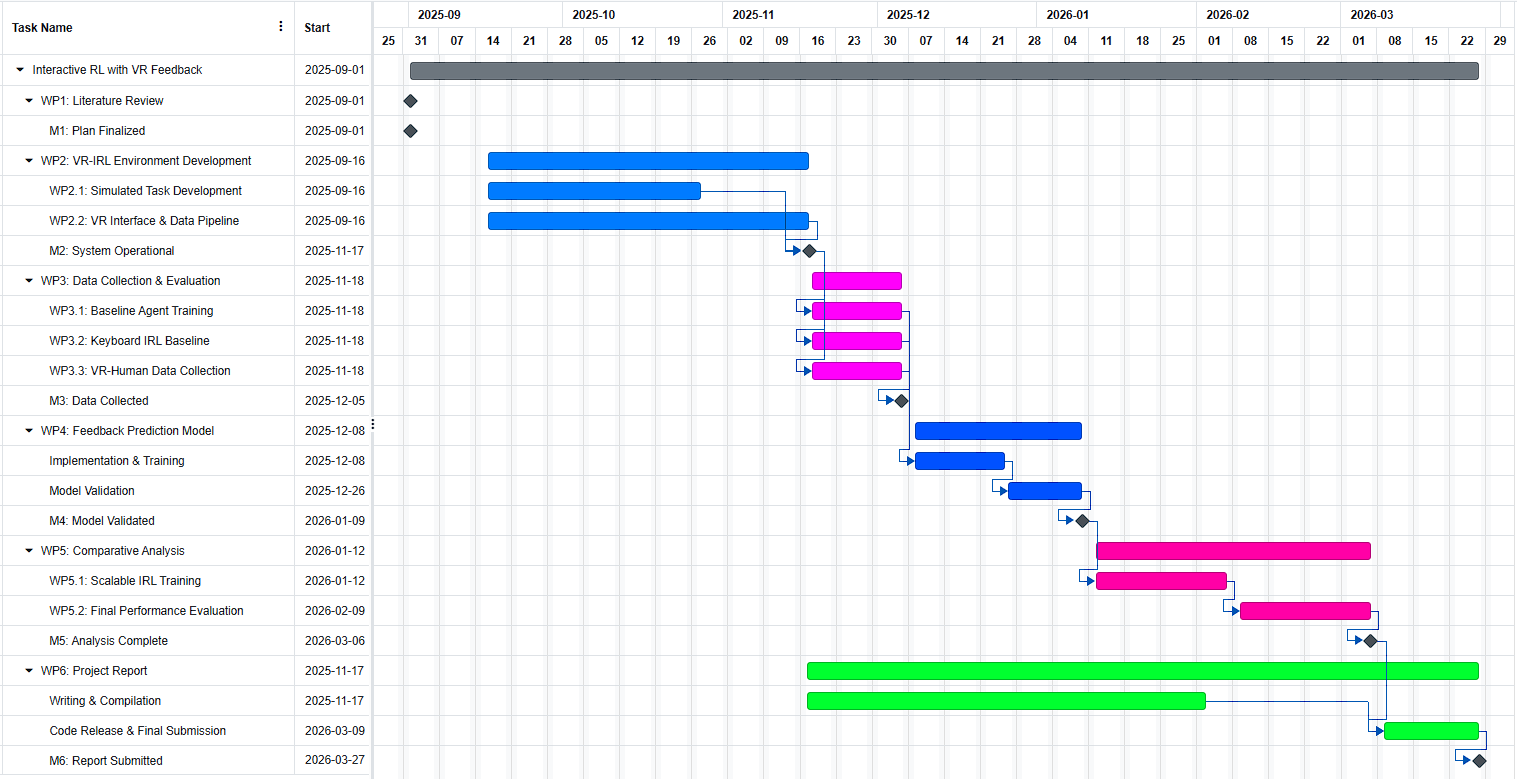
\includegraphics[width=\textwidth]{images/Behrouz_ganttchart}
    \caption{Project schedule Gantt chart, showing the planned duration and overlap of Work Packages (WP1-WP6) and the key Milestones (M1-M6). The OnlineGantt web application (www.onlinegantt.com) was used to create this Chart}
    \label{fig:project_timeline}
\end{figure}

\subsection{Deliverables}

\subsubsection*{Minimum Viable}
\begin{itemize}
    \item A functional Unity VR environment for one simple task (e.g., target reaching).
    \item A basic keyboard-based IRL interface.
    \item A trained baseline RL agent.
    \item A final report documenting the implemented system and baseline results.
\end{itemize}


\subsubsection*{Expected}
\begin{itemize}
    \item All Minimum Viable deliverables, plus:
    \item A fully operational VR-based feedback system for all defined tasks.
    \item A collected dataset of human VR feedback.
    \item A trained keyboard IRL agent and a human-VR IRL agent, with a quantitative comparison showing improved sample efficiency of VR feedback over the keyboard baseline.
    \item A final report with clear analysis and conclusions.
\end{itemize}


\subsubsection*{Desired}
\begin{itemize}
    \item All Expected deliverables, plus:
    \item A successfully trained and validated VR Feedback Model that accurately mimics human feedback.
    \item Results from the scalable synthetic feedback training, demonstrating that the model-based approach can match or outperform training with the human directly in the loop.
    \item A well-documented, open-sourced code repository to support future research.
\end{itemize}

\vspace{10pt}

\begin{itemize}
    \item D1: Literature survey report. (From WP1)
    \item D2: A working Unity VR application for IRL feedback collection. (From WP2)
    \item D3: A dataset of human VR feedback for specified tasks. (From WP3)
    \item D4: Trained VR Feedback Models. (From WP4)
    \item D5: Complete evaluation results (learning curves, performance scores) comparing all training methods. (From WP5)
    \item D6: Final project report and code repository. (From WP6)

\end{itemize}


\nocite{*}

\bibliographystyle{plainnat} % Use the plainnat bibliography style
\bibliography{bibliography.bib} % Use the bibliography.bib file as the source of references

\end{document}
